\paragraph{Register File}

\begin{figure}[H]
    \centering
    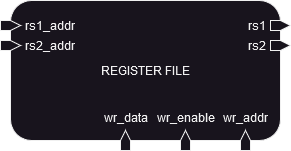
\includegraphics[width=0.5\textwidth]{design/pipelined/rom_ram_reg/images/register_file.png}
    \caption{Register File}
    \label{fig:register_file}
\end{figure}

The register file is a one-cycle really small memory. The RV32I standard requires 32 registers, each 32 bits long. Only the first (zero) register
has a given value of 0, the other can be used at will but as with any other architecture there are some standards for what a register is being used 
for.

Signals:
\begin{enumerate}[label={\textbullet}]
    \item Input: $rs1\_addr$, This signal gives the address of the first register that needs to be read.
    \item Input: $rs2\_addr$, This signal gives the address of the second register that needs to be read.
    \item Input: $wr\_addr$, This signal gives the address of the register that needs to be written.
    \item Input: $wr\_data$, This signal gives the data that needs to be written in the memory.
    \item Input: $wr\_enable$, This signal indicates whether the register should be written with the $wr\_data$ value.
    \item Output: $rs1$, This signal gives the value read at address $rs1\_addr$.
    \item Output: $rs2$, This signal gives the value read at address $rs2\_addr$.
\end{enumerate}